\section{函数重载}
C++中的运算符可以接收不同类型的操作数。\lstinline@.1+.2@,这里的操作数都是 \lstinline@double@ 类型的;\lstinline@1+2@,这里的操作数都是 \lstinline@int@ 类型的;\lstinline@1ll+2ll@,这里的操作数都是 \lstinline@long long@ 类型的(还记得吗,整数带 \lstinline@ll@ 后缀将是 \lstinline@long long@ 类型的。)我们希望同一个函数也能像运算符哪样,支持多种类型。比如 \lstinline@max@ 吧,它是否既可以支持 \lstinline@double@ 类型又可以支持 \lstinline@int@ 类型呢?\par
这种可能性是完全存在的。想想吧,当我们调用函数时,编译器能知道的信息只有函数名和实参——而实参能够提供``参数类型''这则信息。因此我们如果定义一个``接收不同类型参数''的同名函数,编译器仍然可以分得清。\par
当然这只是可行性分析,不代表该语言能允许我们这样做——C语言就不支持这种方法。不过好消息是,C++支持这种方法,它叫做\textbf{函数重载(Function overloading)}。\par
要重载一个函数是非常简单的,只要你用同一个函数名写不一样的参数列表就行了。举例来说,我们在上一节中定义了 \lstinline@max3@,其实我们可以直接用 \lstinline@max@ 这个名字,它就是对原来 \lstinline@max@ 的重载。
\begin{lstlisting}
long long max(long long, long long); //本行代码是非必需的
long long max(long long, long long, long long); //此重载max接收三个long long参数
int main() {
    long long a, b, c;
    cin >> a >> b >> c;
    cout << max(a, b, c); //编译器自动找到max(long long,long long,long long)
    return 0;
}
long long max(long long a, long long b) {
    //省略
}
long long max(long long a, long long b, long long c) {
    //省略
}
\end{lstlisting}
我们还可以重载 \lstinline@double@ 版本的两数 \lstinline@max@ 函数和三数 \lstinline@max@ 函数,只需要在上面的代码中再添加:
\begin{lstlisting}
\\声明部分如下
double max(double, double); //此重载接收两个double参数
double max(double, double, double); //此重载接收三个double参数
\\定义部分如下
double max(double a, double b) {
    if (a > b) {
        return a;
    }
    else {
        return b;
    }
}
double max(double a, double b, double c) {
    const double max_ab {max(a,b)};
    //这里编译器会调用max(double,double)而非max(long long,long long)
    if (max_ab > c) {
        return max_ab;
    }
    else {
        return c;
    }
}
\end{lstlisting}
图4.4即 \lstinline@max@ 函数的四种重载方案。每种重载方案都可以视为一个独立的函数,只是它们名字不同而已。\par
\begin{figure}[htbp]
    \centering
    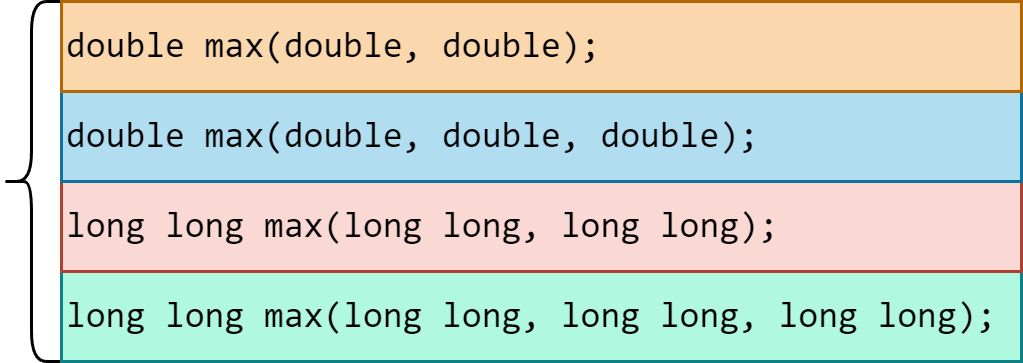
\includegraphics[width=0.6\textwidth]{../images/generalized_parts/04_function_overloading.png}
    \caption{\lstinline@max@ 函数的重载}
\end{figure}
注意,同一个函数的返回类型不能重载。我们写成这样是不行的:
\begin{lstlisting}
//声明部分如下
double max(double,double);
long double max(double,double);
//error: ambiguating new declaration of 'long double max(double, double)'
\end{lstlisting}
编译器的报错信息意为:``\lstinline@long double max(double,double)@ 的定义会引发歧义。''这不难理解。因为在调用函数的时候我们无法指定这个函数的返回类型,所以一旦我们定义了两个完全相同的函数——除了它们的返回类型不同以外,编译器就不可能把它们分开。这就是一种\textbf{二义性(Ambiguity)}。\par
二义性说白了就是歧义。我们日常使用的语言不可避免地会有歧义,但大多数时候我们都能根据实际情况来判断状况,而不致造成错误理解(但这种情况还是时常发生,不是吗)。编译器不具备人的理解能力,它面对二义性问题时无法判断程序员的真实意图,所以只会报错。\par
在涉及到重载时,还有很多种情况会导致二义性的发生,比如这个:
\begin{lstlisting}
void fun(long long); //声明了一个接收long long型变量的函数fun,定义省略
void fun(double); //声明了一个接收double型变量的函数fun,定义省略
int main() {
    fun(1ll, 1.); //实参分别是long long类型和double类型,如何是好?
//(GCC) error: call of overloaded 'fun(long long int, double)' is ambiguous
//(MSVC) error C2666: 'fun': overloaded functions have similar conversions
//(clang) error: call to 'fun' is ambiguous
}
\end{lstlisting}
先不看编译器的报错信息,我们来分析一下这段代码的行为。我们重载了 \lstinline@fun@ 函数,其中一个版本可以接收 \lstinline@long long@ 类型的参数,而另一个版本可以接收 \lstinline@double@ 类型的参数。在主函数中,我向 \lstinline@fun@ 中传入了两个参数,分别是 \lstinline@long long@ 型的 \lstinline@1ll@ 和 \lstinline@double@ 型的 \lstinline@1.@。现在问题来了,编译器究竟是会把 \lstinline@1ll@ 隐式转换成 \lstinline@double@ 类型,还是会把 \lstinline@1.@ 隐式转换成 \lstinline@long long@ 类型呢?\par
编译一下就会发现,无论是GCC,Visual C++还是Clang,都会给出类似于歧义的报错。其中MSVC的报错提到了``have similar conversions'',这正是问题的根源:``把 \lstinline@1ll@ 转换为 \lstinline@double@''或者``把 \lstinline@1.@ 转换成 \lstinline@long long@''都是可行的,这两种方案高度相似,编译器也无法决定怎么转换,于是就出现了二义性问题。\par
怎么解决呢?我们可以使用强制类型转换的方法来把一个参数转换成别的类型,比如都转换成 \lstinline@double@,这样编译器就能直接找到匹配的函数了。\par
还有一种方式就是再定义一个 \lstinline@fun(long long,double)@ 重载函数。但是这样就别提有多麻烦了——那我们是不是还要考虑定义一个 \lstinline@fun(double,long long)@,以防有人使用 \lstinline@fun(1.,1ll)@ 呢?这样的麻烦无穷无尽,那是很烦人的。\footnote{所以你就能理解为什么我们需要泛型编程了,详见本章第六节。}况且,因为 \lstinline@int@ 既可以转换为 \lstinline@double@ 又可以转换为 \lstinline@long long@,那么在调用 \lstinline@max(1,2)@ 时也会出现``编译器不知该使用哪个重载''的二义性问题,那么我们还要再定义 \lstinline@int max(int,int)@(以及各种变形)咯?\par
不过这仅是出于语法层面的考量而言的。实际编程中我们大多会使用同一类型的数据来求最大值,所以只需要定义两(三)个同类型参数的重载,就足以应付大多数需求了。至于更细致的知识,尤其是有关编译器如何处理``类型转换''和``匹配哪个函数''的问题,其实非常复杂,本章不再赘述。我们会在泛讲篇中更深入地探讨这个问题。\par
